\documentclass[12pt]{article}
\usepackage{amsmath}
\usepackage[margin=2cm]{geometry}
\usepackage{graphicx}
\usepackage[utf8]{inputenc}
\graphicspath{ {./img/} }
\DeclareGraphicsExtensions{.png, .jpg, .jpeg}
\begin{document}
\begin{center}
\textbf{Physics Lab \#10: Diffraction Gratings and Laser Diffraction}\\
Charlie Coleman\\
Lab Partners: Alex Bielewicz, Tracey Jaron\\
2016 November 09
\end{center}
\paragraph{Abstract:} The purpose of this lab was to measure the wavelength of various colors of light using a diffraction grating and a measuring the angle of diffraction. Next, the wavelength of a laser was measured using a diffraction setup with multiple slit configurations. This lab heavily utilized the wave behavior of light, taking advantage of constructive and destructive interference to find minimums and maximums of the projected light. The geometry of the diffraction grating gave us the equation $\delta = n \lambda = S sin(\theta_n)$ for the first part, and $bc = \lambda = ab \times sin(\theta)$ and $n \lambda = d sin(\theta)$ for the second part. Using the information in the theory and given here, the wavelengths were found in part one to all be within 20\% of the actual value. This means that this part of the lab was a success. For part two, the wavelength found for the laser did not fall within the given range, so this part of the lab was not a success.

\paragraph{Theory:}\mbox{} \\
\textbf{Part one:}
For part one of this lab, the wavelength of light, $\lambda$, can be found using a diffraction grating of the transmission type using $\delta = n \lambda = S sin \theta_n$ where S is the distance between the grating rulings, $\theta$ is the diffraction angle, and n is the order number. Constructive interference occurs when the difference in path length ($\delta$) is equal to a multiple of the wavelength ($\lambda$). This is the way the colors are spread apart, as the different wavelengths mean that the position for the constructive interference is different for each color. \mbox{} \\ \mbox{} \\
\textbf{Part two:}
\begin{center}
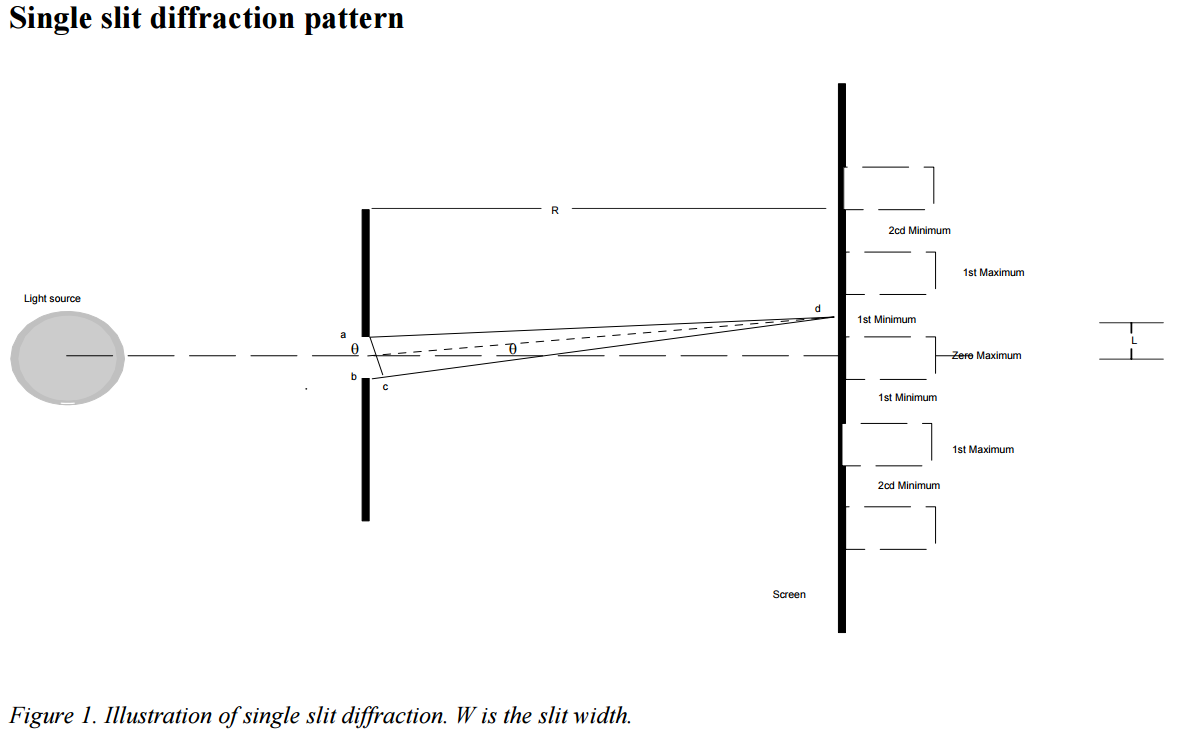
\includegraphics[width=17cm]{singleslit_part2.png}
\end{center}

For part two, the properties of light as a wave must be examined. In the graphic above, the light leaving from point b has traveled farther than light that left from point a when both rays hit point d. If the distance bd is greater than the distance ad by a full wavelength, the waves are said to be in-phase. This means that the waves will add up constructively. Therefore, the waves can be paired so that they reach point d out of phase. When all the waves are added together a dark spot will occur. In this figure, point d makes an angle $\theta$ with respect to the slit and a perpendicular line is drawn from the screen. By geometry, the angle bca is the same as the angle $\theta$. The distance bc must be equal to a full wavelength, $\lambda$, for destructive interference. By trigonometry, we get the equation $ bc= \lambda = ab *sin(\theta)$. As shown in the figure above, there are multiple dark spots. To reach the second minimum, bc must be equal to $2*\lambda$, and for the nth dark spot, bc must be equal to $n*\lambda$. With this information, the equation for the dark spot can be rewritten as $ n \lambda = w sin(\theta)$ where w is the slit width, $\lambda$ is the wavelength, $\theta$ is the angle in the figure, and n is the order of the dark fringe. The equations defines the locations were dark spots are expected.

\begin{center}
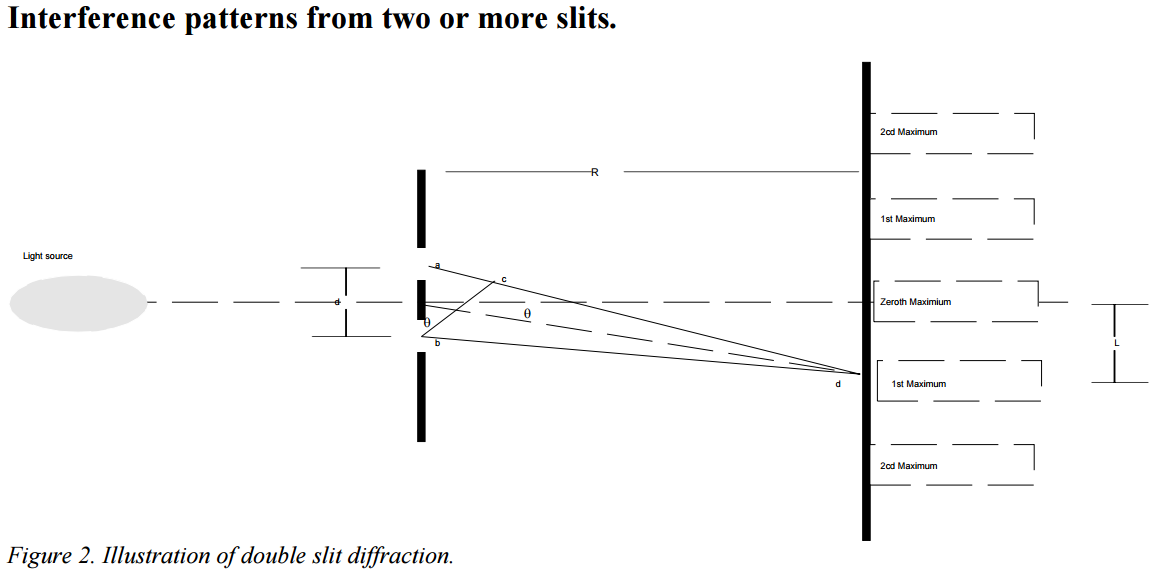
\includegraphics[width=17cm]{multislit_part2.png}
\end{center}

When there are two or more slits, the waves will add up to give minimums and maximums. As shown in the illustration above, the distance that a wave travels along ad is longer than the distance bd. If the difference, ac, is one wavelength, $\lambda$, then the two waves will constructively interfere and create a maximum. The equation for the constructive interference is given as $n \lambda = d sin(\theta)$ where n is the order of the maximum, $\lambda$ is the wavelength, d is the separation of the slits, and $\theta$ is the angle of incidence. 

\paragraph{Objective:} The objective of this lab was to measure the wavelength of light using a diffraction grating and to demonstrate diffraction using a laser and different slit configurations.

\paragraph{Procedure:}

\subparagraph{Part one:} First, clamp the grating in place on the spectrometer table so that it is perpendicular to the collimator axis as shown in the diagram. Next, swing the telescope around so that it is in line with the direct line OM. Record the reading on the vernier scale. Move the telescope away from the direct ray until a spectral line appears. Record the angle. Move the telescope to the other side of the direct line and look for the same spectral line as before. Record the angle. Repeat for multiple spectral lines. Repeat all of that for a second set of spectral lines.

\subparagraph{Part two:} First, point the laser so that the light is projected through the diffraction pattern wheel onto the screen behind. Measure and record the interference pattern spacing and the distance between the pattern and the slit wheel. Do the measurements for the single slit, double slit, and multiple slit openings on the slit wheel. Measure dark spots on the single slit and bright spots on all others.

\paragraph{Setup:}

\subparagraph{Part one:}
\begin{center}
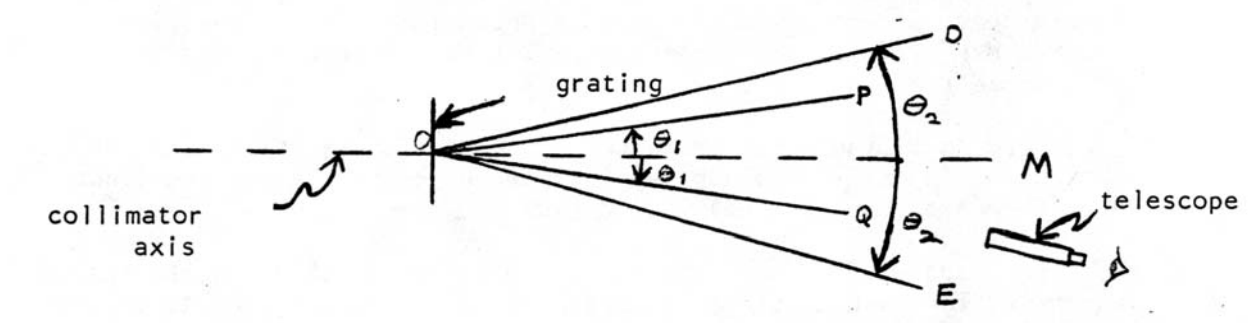
\includegraphics[width=14cm]{apparatus_part1.png}
\end{center}

\subparagraph{Part two:}
\begin{center}
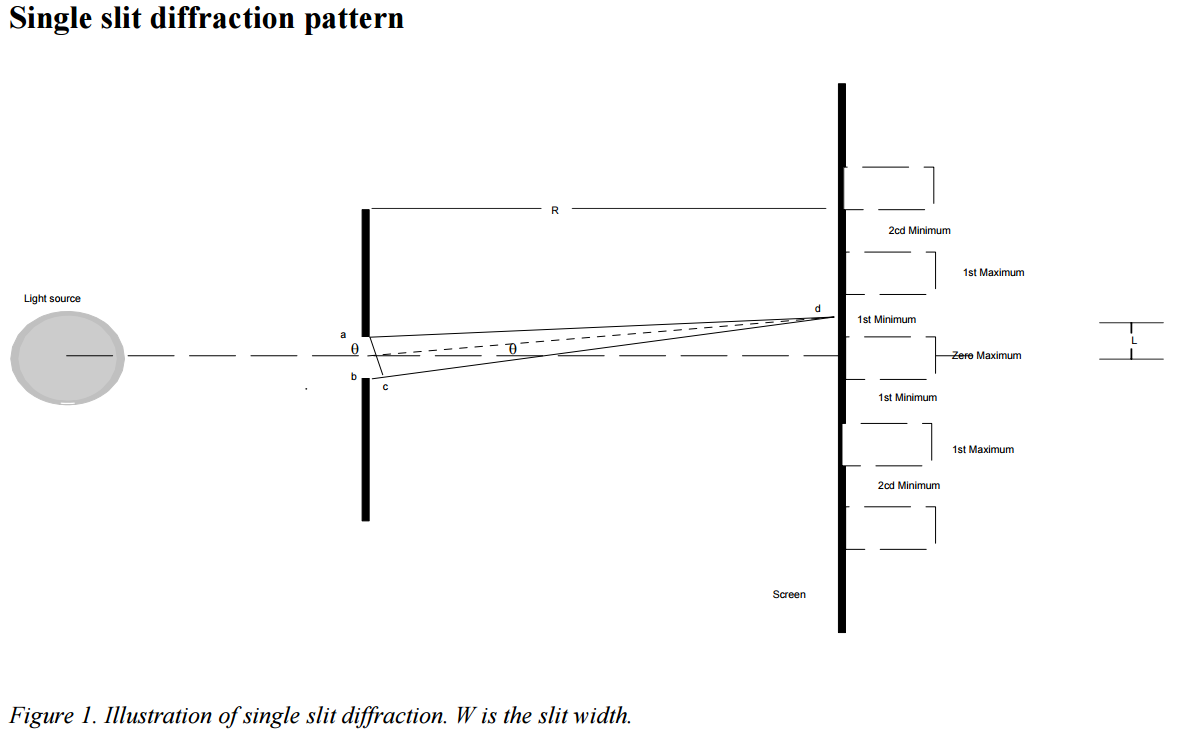
\includegraphics[width=14cm]{singleslit_part2.png}

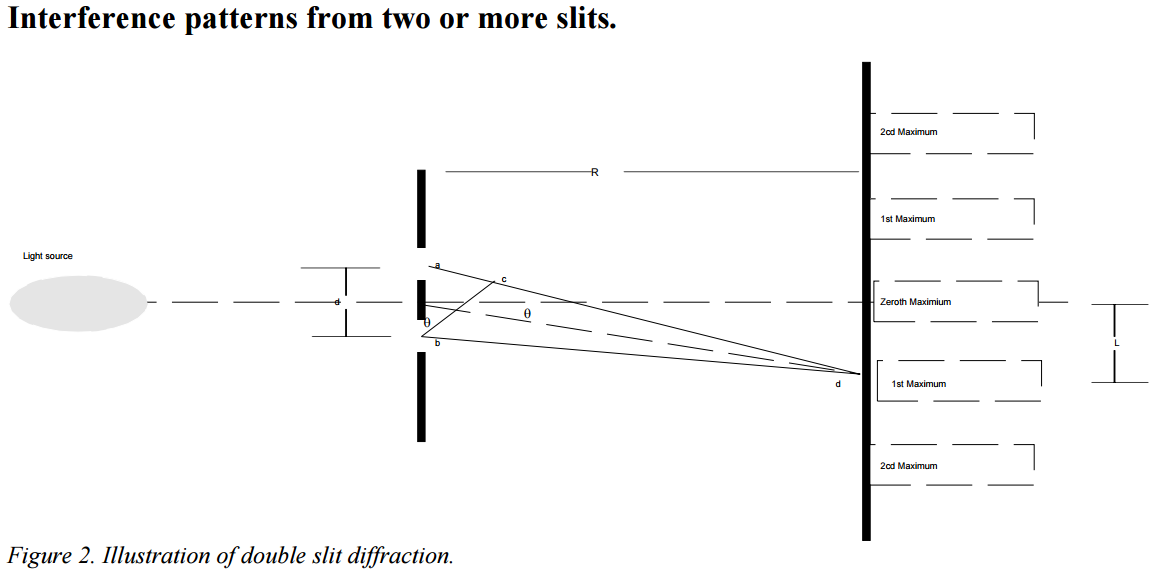
\includegraphics[width=14cm]{multislit_part2.png}
\end{center}

\paragraph{Data:} \mbox{} \\
Part one:
\begin{tabular}{| l | l | c | r |}
	\hline
	Element & Angle & n & Color \\ \hline
	Helium & 19 & 2 & orange \\
	& 15 & 2 & green \\
	& 14.7 & 2 & blue-green \\
	& 14 & 2 & blue-green \\
	& 13.4 & 2 & blue \\
	& 0 & 1 & orange \\
	& 21 & 2 & red \\ \hline
	Mercury & 0 & 1 & green \\
	& 14.3 & 2 & blue \\
	& 18 & 2 & green \\
	& 19.2 & 2 & orange \\ \hline
\end{tabular}
\mbox{} \\
Part two:
\begin{tabular}{| l | l | l | l | l |}
	\hline
	\# of slits & L (m) & R (m) & w & d \\ \hline
	1 & 8.00E-03 & 0.50 & 4.00E-04 & N/A \\
	2 & 1.25E-03 & 0.50 & 4.00E-04 & 2.50E-04 \\
	3 & 1.67E-03 & 0.50 & 4.00E-04 & 1.25E-04 \\
	4 & 2.00E-03 & 0.50 & 4.00E-04 & 1.25E-04 \\
	5 & 2.22E-03 & 0.50 & 4.00E-04 & 1.25E-04 \\ \hline
\end{tabular}


\paragraph{Calculations:} \mbox{} \\
Part one:
\begin{equation*}
\lambda = \frac{d \times sin(\theta)}{n} = \frac{0.0002m * sin(19^\circ)}{2} = 6.511 \times 10^{-5} m
\end{equation*}
\mbox{} \\
Part two:
\begin{equation*}
\theta = tan^{-1} (\frac{L}{R}) = tan^{-1} (\frac{0.008m}{0.50m}) = 0.917^{\circ}
\end{equation*}
\begin{equation*}
\lambda = d*sin(\theta) = 0.00004m * sin(0.917^\circ) = 3.17 \times 10^{-4}m
\end{equation*}


\paragraph{Qualitative Error Analysis:} One error in part one of this lab was the difficulty in reading the angle on the table. The flashlight would cause glare and it was difficult to tell exactly where the line was showing up. This could cause the angle measured to be off and all other calculations would be affected. One error present in part two of this lab was the difficulty in measuring the bright and dark spots. This is because the transition between light and dark was gradual, so the exact brightest or darkest point was hard to find. This means that the distances could have been off, affecting the calculations.

\paragraph{Quantitative Error Analysis:} \mbox{} \\
Part one:
\begin{tabular}{| l | r |}
	\hline
	Element & Percent Error \\ \hline
	Helium & 8.50\% \\
	& 4.91\% \\
	& 7.14\% \\
	& 2.59\% \\
	& 3.54\% \\
	& 0\% \\
	& 1.43\% \\	\hline
	Mercury & 0\% \\
	& 11.78\% \\
	& 11.64\% \\
	&  6.47\% \\ \hline
\end{tabular} \mbox{} \\
Part two: \mbox{} \\
Error range: 
$6.05 \times 10^{-7}m \leq \lambda \leq 6.65 \times 10^{-7}m$
Values: \mbox{} \\
$\lambda_1 = 3.17 \times 10^{-4}m$ \mbox{} \\
$\lambda_2 = 3.57 \times 10^{-5}m$ \mbox{} \\
$\lambda_3 = 2.38 \times 10^{-5}m$ \mbox{} \\
$\lambda_4 = 2.84 \times 10^{-5}m$ \mbox{} \\
$\lambda_5 = 3.15 \times 10^{-5}m$
\paragraph{Results:} \mbox{} \\
Part one:
\begin{tabular}{| l | c | c | r |}
	\hline
	Element & Calculated $\lambda$ & Real $\lambda$ & \% Error \\ \hline
	Helium & 6.511E-05 & 7.065E-05 & 8.50\% \\
	& 5.176E-05 & 4.922E-05 & 4.91\% \\
	& 5.075E-05 & 4.713E-05 & 7.14\% \\
	& 4.838E-05 & 4.713E-05 & 2.59\% \\
	& 4.635E-05 & 4.471E-05 & 3.54\% \\
	& 0 & 0 & 0\% \\
	& 7.167E-05 & 7.065E-05 & 1.43\% \\	\hline
	Mercury & 0 & 0 & 0\% \\
	& 4.940E-05 & 4.358E-05 & 11.78\% \\
	& 6.180E-05 & 5.461E-05 & 11.64\% \\
	& 6.577E-05 & 6.152E-05 &  6.47\% \\ \hline
\end{tabular} \mbox{} \\
Part two:
\begin{tabular}{| l | r |}
	\hline
	\# of slits & $\lambda$ \\ \hline
	1 & 3.17E-04 \\
	2 & 3.57E-04 \\
	3 & 2.38E-05 \\
	4 & 2.84E-05 \\
	5 & 3.15E-05 \\ \hline
\end{tabular}

\paragraph{Conclusion:} The objective of the first part of this lab was to measure the wavelength of light using a diffraction grating. The purpose of part two was to demonstrate diffraction using a laser and multiple different slit configurations. In the first part, the recorded angles and colors of spectral lines were used to calculated the wavelength of light, which was then compared to known wavelengths of different colors of light. Every wavelength calculated in part one was within 20\% of the expected value, and therefore that part of the lab was a success. For part two of the lab, the wavelength of a laser beam was found by recording the distances between minimums and maximums created by shining the light through a diffraction grating of known slit width and slit distance. These data points were used to find the wavelength. None of the wavelengths found fell within the range given in the lab, and therefore this lab was not a success.
\end{document}